%=====================================================================
%	UCT-MARIS-ARU LaTeX THESIS TEMPLATE
%---------------------------------------------------------------------
%	Created by:		R.A. Verrinder
%	Date Modified:	July 2025
%---------------------------------------------------------------------
%	Compile with:	pdfLaTeX
%====================================================================
% UCT thesis guidelines
%---------------------------------------------------------------------
% * The document should include:
%		-	Title Page
%		-	Abstract
%		-	Acknowledgements
%		-	Table of Contents
%		-	List of Figures
%		-	List of Tables
%		-	Chapters
%		-	Bibliography
%		-	Appendices (if any)
%=====================================================================
%	Document properties:
%---------------------------------------------------------------------
%	Paper size:			A4
%	Margins:			1.5 cm (top,bottom,left,right)
%	Printing:			Double sided
%	Base font size:		10pt
%	Paragraph spacing:	10pt
%	Paragraph indent:	0pt
%=====================================================================
\documentclass[a4paper,11pt,oneside]{book}
%---------------------------------------------------------------------
%	PACKAGES
%---------------------------------------------------------------------
%---------------------------------------------------------------------
% BASIC DOCUMENT CONFIGURATION
%---------------------------------------------------------------------
\usepackage[T1]{fontenc}              % Modern font encoding
\usepackage[british]{babel}            % British English hyphenation and dates
\usepackage{setspace}                 % Line spacing commands

%---------------------------------------------------------------------
% PAGE LAYOUT AND STRUCTURE
%---------------------------------------------------------------------
\usepackage[margin=1.5cm]{geometry}   % Page margins
\usepackage{scrextend}                % Extended layout tools
\usepackage{titlesec}                 % Section title formatting
\usepackage{fancyhdr}                 % Headers and footers
\usepackage{lastpage}                 % Reference to last page
\usepackage[bottom]{footmisc}         % Footnotes aligned to bottom
\usepackage{tocloft}                  % TOC customisation
\usepackage{import}                   % Import files/folders
\usepackage{pdfpages}                 % Insert full PDFs
\usepackage{calc}                     % Length arithmetic
\usepackage{xspace}                   % Smarter spacing after macros
\usepackage{datetime}                 % Legacy date formatting
\usepackage[en-GB]{datetime2}         % Date formatting.
                                     % NOTE: en-GB is a datetime2 locale.
                                     % babel does NOT accept it: babel wants
                                     % "british", as set above.
                                     % NOTE: en-GB is a datetime2 locale.
                                     % babel does NOT accept it: babel wants
                                     % "british", as set above. Passing en-GB
                                     % to babel raises
                                     %   ! Package babel Error: Unknown option
                                     % NOTE: en-GB is a datetime2 locale.
                                     % babel does NOT accept it: babel wants
                                     % "british", as set above. Passing en-GB
                                     % to babel raises
                                     %   ! Package babel Error: Unknown option
\DTMlangsetup[en-GB]{ord=omit}        % Remove 'st', 'nd' etc. from dates
\usepackage[nonumberlist]{glossaries} % Glossary without page numbers

%---------------------------------------------------------------------
% FONTS AND TYPOGRAPHY
%---------------------------------------------------------------------
\usepackage{fix-cm}                  % Enable scalable font sizes
\usepackage{color}                   % Basic colour support
\usepackage[dvipsnames,table,xcdraw]{xcolor} % Extended colours
\usepackage{gensymb}                 % Generic symbols (e.g. °)
\usepackage{ebgaramond}    % Use EB Garamond font

%---------------------------------------------------------------------
% GRAPHICS AND VISUALS
%---------------------------------------------------------------------
\usepackage{graphicx}                % Image inclusion
\usepackage{float}                   % Improved float positioning
\usepackage{wrapfig}                 % Wrap text around figures
\usepackage{lscape}                  % Landscape pages
\usepackage{rotating}                % Rotated figures/tables
\usepackage{subcaption}              % Sub-figures support
\usepackage{caption}                 % Caption formatting
\usepackage{tikz}                    % Create vector graphics
\usepackage{mdframed}                % Framed text boxes

%---------------------------------------------------------------------
% TABLES
%---------------------------------------------------------------------
\usepackage{array}                   % Custom column formatting
\usepackage{booktabs}                % High-quality table lines
\usepackage{tabularx}                % Tables with flexible width
\usepackage{multirow}                % Multirow table cells
\usepackage{hhline}                  % Fine-tuned horizontal lines

%---------------------------------------------------------------------
% LISTS AND ENUMERATION
%---------------------------------------------------------------------
\usepackage{enumitem}                % Custom list formatting

%---------------------------------------------------------------------
% TEXT ALIGNMENT AND JUSTIFICATION
%---------------------------------------------------------------------
\usepackage{ragged2e}                % Better text justification
\usepackage{hyphenat}                % Hyphenation control

%---------------------------------------------------------------------
% REFERENCES, CITATIONS, AND LINKS
%---------------------------------------------------------------------
\usepackage{hyperref}                % Hyperlinks in PDF
%---------------------------------------------------------------------
%   hidelinks removes the coloured boxes hyperref draws around every link,
%   reference and URL. They are invisible on screen in some viewers and
%   print as boxes on paper, which looks like a mistake in a bound thesis.
%
%   If you WANT coloured links (for a screen-only PDF), replace hidelinks
%   with e.g.
%       \hypersetup{colorlinks=true, linkcolor=blue, citecolor=blue,
%                   urlcolor=blue}
%---------------------------------------------------------------------
\hypersetup{hidelinks}
\usepackage{fancyref}                % Enhanced references
\usepackage{url}                     % URL formatting
%=====================================================================
%   CITATION STYLE
%=====================================================================
%   ONE SWITCH. Set it here and both the in-text citations and the
%   bibliography follow.
%
%       \IEEEcitefalse   Harvard   (Shannon, 1948)   <- default
%       \IEEEcitetrue    IEEE      [1]
%
%   The declaration page commits you to the Harvard convention, so leave
%   this false unless you have changed the declaration as well.
%
%   NOTE ON THE SQUARE BRACKETS: natbib loaded with NO options defaults to
%   NUMERIC citations, which is where [1] comes from. It has to be told
%   "authoryear" explicitly, even when the .bst is an author-year style.
%   The two are configured separately and will not agree on their own.
%=====================================================================
\newif\ifIEEEcite
\IEEEcitefalse

\ifIEEEcite
    % IEEE: numeric, square brackets, sorted and compressed ([1]-[3], not [1],[2],[3])
    \PassOptionsToPackage{numbers,square,comma,sort&compress}{natbib}
\else
    % Harvard: author-year, round brackets, semicolon between citations
    \PassOptionsToPackage{authoryear,round,semicolon}{natbib}
\fi
\usepackage{natbib}
%=====================================================================
\usepackage{refcount}                % Arithmetic on \pageref values, for the
                                     % automatic page count on the declaration

%---------------------------------------------------------------------
% VERBATIM AND CODE LISTINGS
%---------------------------------------------------------------------
\usepackage{fancyvrb}                % Code-style text environments

%---------------------------------------------------------------------
% MATHS
%---------------------------------------------------------------------
\usepackage{amsmath, amsthm, amssymb} % Core maths packages
\usepackage{bm}                       % Bold maths symbols

%---------------------------------------------------------------------
% GLOSSARY DEFINITIONS
%---------------------------------------------------------------------

%=====================================================================
%   AUTOMATIC WORD AND PAGE COUNT
%=====================================================================
%   The declaration page states a word count and a page count, EXCLUDING the
%   preamble, the appendices and the bibliography. Both are computed rather
%   than typed, so they cannot go stale the moment you add a paragraph.
%
%   PAGE COUNT
%     \label{body:start} is placed just before the first body chapter and
%     \label{body:end} just after the last one. \bodypages is the difference,
%     using \getpagerefnumber from refcount. It needs TWO LaTeX passes, like
%     any cross-reference. On the first pass it prints ??.
%
%   WORD COUNT
%     LaTeX cannot count words: by the time it sees the text it has already
%     thrown away the distinction between a word and a macro argument. The
%     count is therefore produced OUTSIDE the document, by texcount, and
%     written to wordcount.tex, which is read back in here.
%
%     latexmkrc runs it before each build. If it has not run, the placeholder
%     below is printed instead, so the thesis still compiles.
%=====================================================================
\providecommand{\wordcount}{\textcolor{red}{[run latexmk]}}

%   NOTE the file name. It is NOT "wordcount.tex": TeX Live already ships a
%   file by that name (an interactive word-counting utility). If the generated
%   file is missing, \InputIfFileExists{wordcount} finds TeX Live's copy on the
%   search path instead, runs it, and the build stops dead at
%
%       File name [press RETURN to cancel]:
%       ! Emergency stop.
%
%   which is a baffling thing to debug. The generated file is therefore called
%   thesis-wordcount.tex, which nothing else claims.
\InputIfFileExists{thesis-wordcount.tex}{}{}

\newcommand{\bodypages}{%
    %   The two \pageref calls below are typeset into a box that is then
    %   thrown away, so they print nothing. They are here on purpose.
    %
    %   \getpagerefnumber returns 0 for a label it has not seen yet, and does
    %   so SILENTLY: no warning, because no \ref was used. latexmk therefore
    %   believes the document has converged after one pass and stops, and the
    %   declaration goes out saying
    %
    %       Page count   1 pages
    %
    %   which is 0 - 0 + 1, and is wrong, and looks plausible enough to miss.
    %
    %   Using \pageref makes LaTeX raise its own "Reference undefined" warning
    %   on the first pass, which is what makes latexmk run a second one.
    \begingroup
        \setbox0=\hbox{\pageref{body:start}\pageref{body:end}}%
    \endgroup
    \number\numexpr\getpagerefnumber{body:end}-\getpagerefnumber{body:start}+1\relax
}
%---------------------------------------------------------------------
%=====================================================================

\makeglossaries

%---------------------------------------------------------------------
%   Glossary and acronym entries are DEFINED here, in the preamble.
%   v_glossary.tex only prints the list; it defines nothing.
%---------------------------------------------------------------------
%=====================================================================
%   GLOSSARY AND ACRONYM ENTRIES
%=====================================================================
%   Entries must be DEFINED in the preamble, before they are used. This file
%   is \input from 0_main.tex, after \makeglossaries.
%
%   v_glossary.tex only PRINTS the list. It does not define anything.
%
%   USE
%     \gls{ecsa}    first use  -> Engineering Council of South Africa (ECSA)
%                   after that -> ECSA
%     \glspl{ga}    plural
%     \Gls{ga}      capitalised at the start of a sentence
%
%   An entry that is never cited with \gls does not appear in the list. That
%   is deliberate: the list shows what the reader actually met.
%=====================================================================

%---------------------------------------------------------------------
%   ACRONYMS
%---------------------------------------------------------------------
%   Needed by Appendix D (the ECSA Graduate Attributes table). Leave these.
\newacronym{ecsa}{ECSA}{Engineering Council of South Africa}
\newacronym{ga}{GAs}{Graduate Attributes}

%   Generally useful. Keep or delete.
\newacronym{uct}{UCT}{University of Cape Town}
\newacronym{fyp}{FYP}{Final Year Project}

%   Cited by the example chapters. Replace with your own.
\newacronym{gps}{GPS}{Global Positioning System}
\newacronym{miz}{MIZ}{Marginal Ice Zone}
\newacronym{so}{SO}{Southern Ocean}

%   Add your own below. One line each. They only appear in the printed list
%   if they are actually cited with \gls somewhere.
% \newacronym{adc}{ADC}{analogue-to-digital converter}
% \newacronym{imu}{IMU}{inertial measurement unit}

%---------------------------------------------------------------------
%   GLOSSARY TERMS (a definition, not an abbreviation)
%---------------------------------------------------------------------
% \newglossaryentry{marginalicezone}{
%     name        = {marginal ice zone},
%     description = {The transitional region between the open ocean and
%                    consolidated pack ice, where surface waves and sea ice
%                    interact.}
% }
%=====================================================================

%---------------------------------------------------------------------
%	DOCUMENT
%---------------------------------------------------------------------
\begin{document}
%---------------------------------------------------------------------
%---------------------------------------------------------------------
% Document Properties Macros
%---------------------------------------------------------------------
% Title Information
%---------------------------------------------------------------------
\newcommand{\titl}{Thesis Title}
\newcommand{\subtitle}{Thesis Subtitle}
%---------------------------------------------------------------------
% Degree Information
%---------------------------------------------------------------------
\newcommand{\degreeprogramme}{Electrical Engineering}
%\newcommand{\degreeprogramme}{Electrical and Computer Engineering}
%\newcommand{\degreeprogramme}{Mechatronics}
%\newcommand{\degreeprogramme}{Ocean & Atmosphere Science}
%\newcommand{\degreeprogramme}{Applied Ocean Sciences (Operational Oceanography)}
%\newcommand{\degreee}{Bachelor of Science in \degreeprogramme}
%\newcommand{\degreee}{Bachelor of Science with Honours in \degreeprogramme}
\newcommand{\degreee}{Master of Science in \degreeprogramme}
%\newcommand{\degreee}{Doctor of Philosophy}
%\newcommand{\degreeabv}{BSc (Eng)}
%\newcommand{\degreeabv}{BSc (Hon)}
\newcommand{\degreeabv}{MSc (Eng)}
%\newcommand{\degreeabv}{MSc}
%\newcommand{\degreeabv}{PhD}
%---------------------------------------------------------------------
% Document Type
%---------------------------------------------------------------------
%\newcommand{\documenttype}{final year project report}
\newcommand{\documenttype}{thesis}
%\newcommand{\documenttype}{dissertation}
%---------------------------------------------------------------------
% Author Information
%---------------------------------------------------------------------
\newcommand{\auth}{Glen Oliver \textbf{Jones}}
\newcommand{\studentnumber}{JNSGLE007}
\newcommand{\psemplid}{TODO}
\newcommand{\aemail}{jnsgle007@uct.ac.za}
%---------------------------------------------------------------------
% Identifiers
%---------------------------------------------------------------------
\newcommand{\ebeethicsnumber}{STU-EBE-yyyy-PSQxxxxxx}
%   \href, NOT \hyperlink. \hyperlink jumps to a target INSIDE this document;
%   it does not open a URL. Written with \hyperlink, these two links look
%   right on the page and do nothing when clicked.
\newcommand{\orcidid}{\href{https://orcid.org/xxxx-xxxx-xxxx-xxxx}{xxxx-xxxx-xxxx-xxxx}}
\newcommand{\gitrepo}{\href{https://github.com/username/project}{Repo name}}
%---------------------------------------------------------------------
% Institutional Information
%---------------------------------------------------------------------
\newcommand{\dept}{Department of Electrical Engineering}
%\newcommand{\dept}{Department of Oceanography}
\newcommand{\uni}{University of Cape Town}
\newcommand{\city}{Rondebosch, Cape Town}
\newcommand{\country}{South Africa}

%---------------------------------------------------------------------
% Supervisors
%---------------------------------------------------------------------
\newcommand{\supervisor}{Supervisor's Initials \textbf{Surname}}
\newcommand{\cosupervisor}{Co-supervisor's Initials \textbf{Surname}}
\newcommand{\hod}{Prof. M.A. Khan}
%\newcommand{\hod}{Prof. M. Vichi}
%---------------------------------------------------------------------
% Keywords
%---------------------------------------------------------------------
\newcommand{\key}{keyword1; keyword2; keyword3}
%---------------------------------------------------------------------
% UCT Logos
%---------------------------------------------------------------------
\newcommand{\logo}{
\includegraphics[height=3.5cm]{figs/0_logos/logo_uct.png}}
%---------------------------------------------------------------------
% Research Group Logos
%---------------------------------------------------------------------
%---------------------------------------------------------------------
%   RESEARCH GROUP LOGOS (title page, below the title block)
%---------------------------------------------------------------------
%   Uncomment the groups this thesis actually belongs to. All of them are
%   commented out at present, so \bottomlogos prints nothing and the title
%   page is clean.
%
%   Available in figs/0_logos/:
%       logo_aru.jpg     African Robotics Unit
%       logo_rrsg.png    Radar Remote Sensing Group
%       logo_MARIS.jpg   Marine and Antarctic Research centre (MARiS)
%       logo_MMRU.jpg    Marine Mammal Research Unit
%       logo_socco.png   Southern Ocean Carbon and Climate Observatory
%       logo_SEA.png     SEA
%       logo_eee.jpg     Department of Electrical Engineering
%
%   Keep to three across a row, or they will not fit. If you use fewer than
%   three, widen the minipages so they still balance.
%---------------------------------------------------------------------
\newcommand{\bottomlogos}{
  \begin{figure}[H]
    \begin{minipage}{0.3\textwidth}
      \centering
      % 
\includegraphics[height=2cm]{figs/0_logos/logo_aru.jpg}
    \end{minipage}
    \hfill
    \begin{minipage}{0.3\textwidth}
      \centering
      
\includegraphics[height=2cm]{figs/0_logos/logo_eee.jpg}
    \end{minipage}
    \hfill
    \begin{minipage}{0.3\textwidth}
      \centering
      % 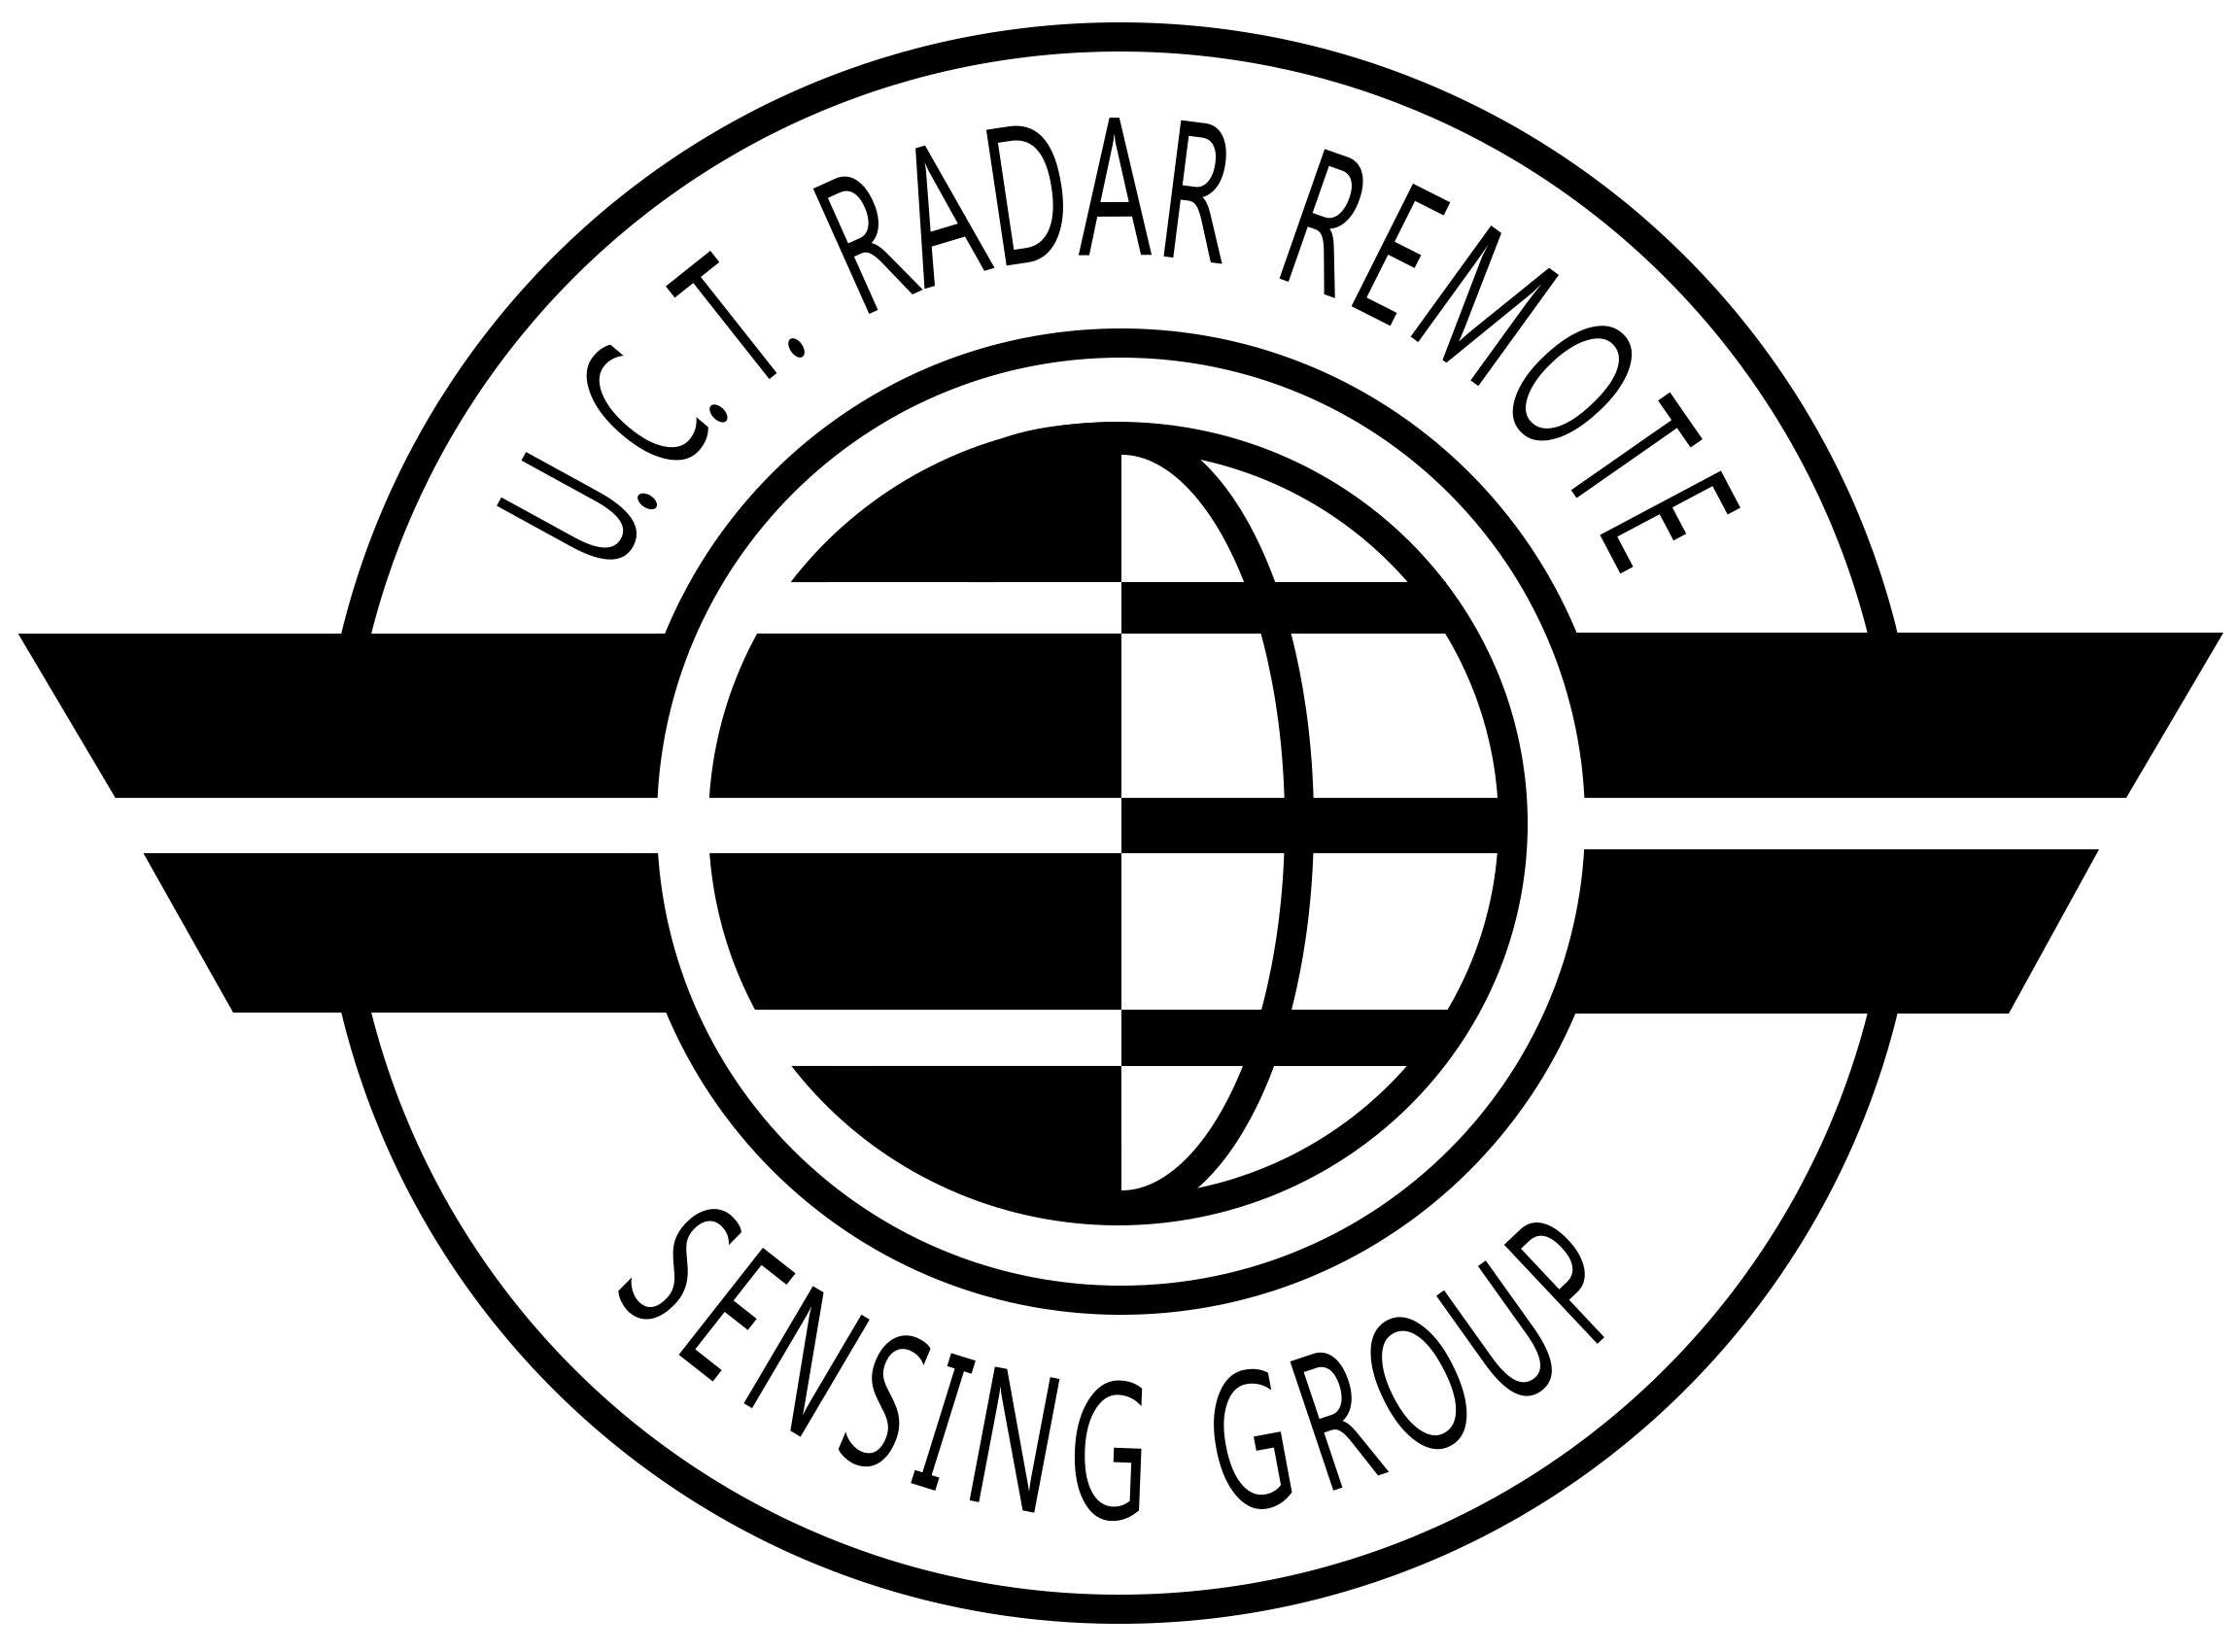
\includegraphics[height=2cm]{figs/0_logos/logo_rrsg.png}
      % 
\includegraphics[height=2cm]{figs/0_logos/logo_MARIS.jpg}
      % 
\includegraphics[height=2cm]{figs/0_logos/logo_MMRU.jpg}
      % 
\includegraphics[height=1.5cm]{figs/0_logos/logo_socco.png}
    \end{minipage}
  \end{figure}
}
%=====================================================================
%	DOCUMENT PROPERTIES
%---------------------------------------------------------------------
% 	PAGE FORMATTING
%---------------------------------------------------------------------
\setlength{\parskip}{10pt}       % Paragraph spacing
\setlength{\parindent}{0pt}      % No paragraph indentation
%---------------------------------------------------------------------
% 	CAPTIONS  Caption margins 80% of text
%---------------------------------------------------------------------
\captionsetup{
  width=0.8\textwidth,
  font=footnotesize,
  labelfont=bf
}                               
%---------------------------------------------------------------------
% 	FOOTNOTES
%---------------------------------------------------------------------
\renewcommand{\thefootnote}{\fnsymbol{footnote}}

%---------------------------------------------------------------------
% Header and Footer
%---------------------------------------------------------------------
\pagestyle{fancy}
\fancyhf{}
\fancyhead[L]{\leftmark}
\fancyhead[R]{\thepage}
\setlength{\footskip}{0.5cm}     % Ensure space for the footer
\setlength{\headheight}{1cm}     % Increase header height
\setlength{\headsep}{0.5cm}      % Increase space between header and text

%---------------------------------------------------------------------
%	NEW COMMANDS
%---------------------------------------------------------------------
% Macros for Date and Time
%---------------------------------------------------------------------
\newcommand{\thesisdate}{\DTMdisplaydate{2024}{07}{01}{-1}}
\newcommand{\FullDate}{\shortdayofweekname{\day}{\month}{\year} \the\day\ \monthname[\month], \the\year}
\newcommand{\MonthYear}{\monthname[\month] \the\year}

%---------------------------------------------------------------------
% Signature Macro
%---------------------------------------------------------------------
\newcommand*{\signature}[1]
{
    \par\noindent\makebox[8cm]{\hrulefill}
    \par\noindent\makebox[8cm][r]{#1}
}

%---------------------------------------------------------------------
% Theorems and Activities
%---------------------------------------------------------------------
\newtheorem*{guess*}{Hypothesis}
\newtheorem*{activity*}{Activity}

%---------------------------------------------------------------------
% Define custom colors
%---------------------------------------------------------------------
\definecolor{titlebg}{HTML}{959595}
\definecolor{colbg}{HTML}{F5F5F5}
\definecolor{objectivebg}{HTML}{C5C5C5}
\definecolor{defaulttext}{HTML}{595959}
\definecolor{tablerule}{HTML}{666666}

%---------------------------------------------------------------------
% 	TOC FORMATTING
%---------------------------------------------------------------------
% Set spacing between entries
\renewcommand{\cftchapfont}{\normalfont\bfseries}
\renewcommand{\cftsecfont}{\normalfont}
\renewcommand{\cftsubsecfont}{\normalfont}
\renewcommand{\cftchappagefont}{\normalfont\bfseries}
\renewcommand{\cftsecpagefont}{\normalfont}
\renewcommand{\cftsubsecpagefont}{\normalfont}
\setlength{\cftbeforechapskip}{5pt}
\setlength{\cftbeforesecskip}{3pt}
\setlength{\cftbeforesubsecskip}{2pt}

% Enable dot leaders
\renewcommand{\cftchapdotsep}{\cftdotsep}
\renewcommand{\cftsecdotsep}{\cftdotsep}
\renewcommand{\cftsubsecdotsep}{\cftdotsep}

% Default: Display "Chapter" in ToC entries for regular chapters
\renewcommand{\cftchappresnum}{\chaptername\space}

% Set ToC entries for appendix chapters to display "Appendix"
\setlength{\cftchapnumwidth}{\widthof{\textbf{Appendix~999~}}}
\makeatletter
\g@addto@macro\appendix{%
  \addtocontents{toc}{%
    \protect\renewcommand{\protect\cftchappresnum}{\appendixname\space}%
  }%
}
\makeatother

% Reduce space before chapter headings
\titlespacing*{\chapter}{0pt}{-10pt}{20pt}

% Adjust chapter heading formatting to avoid cropping
\titleformat{\chapter}[display]
  {\normalfont\huge\bfseries}{\chaptertitlename\ \thechapter}{20pt}{\Huge}
\titlespacing*{\chapter}{0pt}{10pt}{40pt}


\newcolumntype{U}{>{\raggedleft\arraybackslash}p{2cm}}
%=====================================================================
%	TITLE PAGE
%=====================================================================
%=====================================================================
%	TITLE PAGE
%=====================================================================
\begin{titlepage}
    \centering
    \vspace*{1cm}

    % Title
    \begin{Huge}
        \bfseries\titl\par
        \vskip 0.2cm
    \end{Huge}

    % Subtitle
    \begin{Large}
        \subtitle\\*
        \vskip 2cm
    \end{Large}

    % UCT logo
    \logo

    \vskip 2cm

    % Author
    \begin{Large}
        \bfseries\auth\\
    \end{Large}

    % Author's address
    \begin{normalsize}
        \vskip 2mm
        \dept\\*
        \uni\\*
        \city\\*
        \country\\*

        \vskip 1cm
    \end{normalsize}

    % Supervisor (optional)
    \begin{normalsize}
        {\itshape Supervisor \\*}
        \supervisor\\
        \vskip 0.2cm
    \end{normalsize}

    % Cosupervisor (optional)
    \begin{normalsize}
        {\itshape Co-supervisor(s) \\*}
        \cosupervisor\\
        \vskip 1cm
    \end{normalsize}

    % Date
    \begin{Large}
        {\bfseries \MonthYear}
        \vskip 0.5cm
    \end{Large}

    % Degree
    \degreeabv\ \documenttype\ submitted in partial fulfilment of the requirements for the degree of \degreee\ in the \dept\ at the \uni

    \vskip 0.5cm

    % Keywords
    \begin{normalsize}
        {\itshape Keywords:}
        \key
    \end{normalsize}

    \vskip 1cm

    % MARIS and ARU logos
    \bottomlogos
\end{titlepage}

%=====================================================================
%	FRONT MATTER
%=====================================================================
%---------------------------------------------------------------------
%   FRONT MATTER
%---------------------------------------------------------------------
%   \pagestyle{plain} gives the front matter a page number in the footer and
%   NOTHING in the header. The book class defaults to "headings", which puts a
%   running head with the chapter name at the top of every page, which is not
%   wanted on the declaration, the abstract or the contents.
%
%   The running heads are restored at the start of the main matter, so the
%   body chapters keep them.
%---------------------------------------------------------------------
\frontmatter
\pagestyle{plain}
%---------------------------------------------------------------------
%	Declaration
%---------------------------------------------------------------------
%---------------------------------------------------------------------
%	Declaration
%---------------------------------------------------------------------
\chapter{Declaration}
\label{ch:decl}

% In your document body
I, \textbf{\auth}, hereby:

\begin{enumerate}[label=\arabic*.]
    \item know that plagiarism is wrong. Plagiarism is to use another’s work and pretend that it is one’s own.

    \item have used the {\bf Harvard} convention for citation and referencing. Each contribution to, and quotation in, this report from the work(s) of other people has been attributed, and has been cited and referenced. Any section taken from an internet source has been referenced to that source.

    \item declare that: 
    \begin{enumerate}[label=\alph*.]
        \item this report is my own work, and apart from the normal guidance from my supervisor(s), I have received no assistance except as acknowledged.
        
        \item neither the substance nor any part of the above report has been submitted in the past, or is being, or is to be submitted for a degree at this University or at any other university.
        
        \item I have not paid a third party to complete my work on my behalf.
        
        \item my use of artificial intelligence software has been limited to:
        
        \vspace{1em}
        \textbf{\em (specify which tool was used and how you used AI to assist with this project).}
        \vspace{1em}
    \end{enumerate}

    \item have not allowed and will not allow anyone to copy my work with the intention of passing it off as their own work.

    \item acknowledge that copying someone else’s work, or part of it, is wrong, and declare that this is my own work.

    \item grant the University of Cape Town free license to reproduce the above thesis in whole or in part, for the purpose of research.
\end{enumerate}


\vfill % Push the following content to the bottom of the page
%---------------------------------------------------------------------
% WORD COUNT/PAGE COUNT and SIGNATURE
%---------------------------------------------------------------------
\begin{tabularx}{\textwidth}{>{\raggedright\arraybackslash}X>{\raggedleft\arraybackslash}X}
\begin{tabular}{@{}ll@{}}
%   Both counts are computed, not typed. See the AUTOMATIC WORD AND PAGE
%   COUNT block in 0_main.tex. The page count needs two LaTeX passes.
\textbf{Word count} & \wordcount{} words {\footnotesize (excluding preamble, appendices and bibliography)}\\
\textbf{Page count} & \bodypages{} pages {\footnotesize (excluding preamble, appendices and bibliography)} \\
\end{tabular}
&
\begin{minipage}[t]{0.45\textwidth}
    \raggedleft
%   figs/signature.jpg ships as a placeholder X. Replace it with a scan of
%   your own signature before submitting.
%
%   Do NOT commit your real signature back to this template repository, or to
%   any repository other people can clone. Keep it in your own thesis repo,
%   and think about whether that one should be private.
    
\includegraphics[height=1cm]{figs/signature.jpg} % Adjust height as needed
    \vskip 1mm
    \noindent \textbf{\auth} % Author name below the signature
    \vskip 1mm
    {\footnotesize \dept \\*
    \uni \\*}
    \vskip 1mm
    \FullDate
\end{minipage}
\\
\end{tabularx}
        \vspace{2em}
%---------------------------------------------------------------------

%---------------------------------------------------------------------
%	Abstract
%---------------------------------------------------------------------
%---------------------------------------------------------------------
%	Abstract
%---------------------------------------------------------------------
\chapter{Abstract}				
\label{ch:abs}
%---------------------------------------------------------------------
% TAKEN FROM UCT WEBSITE
% The Doctoral Degrees Board recommends that candidates include an abstract 
% that fits onto one page, and which includes the author's full name, thesis 
% title and date. The text should not exceed 350 words. Candidates may also 
% include a more substantial summary of their work, in addition to the abstract.
% Follow the same format for an MSc. abstract.

% The abstract should stand on its own. It should answer the following questions:
%	1.	What did the author do? What ideas, notions, hypotheses, 
%		concepts, theories or thoughts were investigated?
%	2.	How did the author do the work? What data were generated and used? 
%		What was the origin of the data? How were data gathered? 
%		What tests, scales, indices, or summary measures were used? 
%		In other words, how was the analysis and/or synthesis done?
%	3.	What were the conclusions and what were the significant findings?
%
% Some studies cannot readily be summarised in this way and require more 
% descriptive abstracts. Do not use telegraphic phrases. Do not repeat 
% information given in the title. Do not use abbreviations. The purpose of 
% an abstract is to enable a researcher/examiner to understand the essential 
% hypothesis, method and findings of the research.
%---------------------------------------------------------------------
\begin{center}
	\textbf{\Large \titl}\\
			\vskip 0.2cm
			\auth\\
			\vskip 0.2cm
	\textit{\footnotesize \FullDate}
			\vskip 1cm
\end{center}
%---------------------------------------------------------------------
% Write abstract here [350 words]
%---------------------------------------------------------------------

%---------------------------------------------------------------------
%	Acknowledgements
%---------------------------------------------------------------------
%---------------------------------------------------------------------
%	Acknowledgements
%---------------------------------------------------------------------
\chapter{Acknowledgements}		
\label{ch:ack}
%---------------------------------------------------------------------
% Acknowledge all people who have helped you complete this work including.
% Comment out /nrf macro if unneeded.
%---------------------------------------------------------------------
%\nrf

%---------------------------------------------------------------------
%	Dedication (optional)
%---------------------------------------------------------------------
%\begin{flushright}
%	\vspace*{10cm}
%	{\itshape dedication .....}
%\end{flushright}

%---------------------------------------------------------------------
% Table of Contents
%---------------------------------------------------------------------
\tableofcontents
\pagebreak
%---------------------------------------------------------------------
% List of Figures
%---------------------------------------------------------------------
\listoffigures
\addcontentsline{toc}{chapter}{List of Figures}
\pagebreak
%---------------------------------------------------------------------
% List of Tables
%---------------------------------------------------------------------
\listoftables
\addcontentsline{toc}{chapter}{List of Tables}

%---------------------------------------------------------------------
%	List of Symbols/Document conventions (optional)
%---------------------------------------------------------------------
%---------------------------------------------------------------------
%	List of Symbols
%---------------------------------------------------------------------
\chapter{List of Symbols}
%---------------------------------------------------------------------
\label{ch:symbols}
\addcontentsline{toc}{chapter}{List of Symbols}
%---------------------------------------------------------------------
\noindent
\begin{tabularx}{\textwidth}{@{}l X U@{}}
\toprule
\textbf{Symbol} & \textbf{Description} & \textbf{Unit} \\
\midrule
$\bm{B}$         & Magnetic flux density         & T \\
$\bm{E}$         & Electric field                & V/m \\
$\bm{J}$         & Current density               & A/m$^2$ \\
$t$              & Time                          & s \\
$\varepsilon_0$  & Permittivity of free space ($8.85 \times 10^{-12}$) & C$^2$/N·m$^2$ \\
$\mu_0$          & Permeability of free space ($4\pi \times 10^{-7}$)  & N/A$^2$ \\
\bottomrule
\end{tabularx}


%---------------------------------------------------------------------
%	Glossary (optional)
%---------------------------------------------------------------------
%---------------------------------------------------------------------
%	Glossary
%---------------------------------------------------------------------
\printglossary[
     style=list,
% style=listgroup,
     type=\acronymtype,
     title=List of Acronyms and Glossary,
]
%---------------------------------------------------------------------
%\chapter{Glossary}		
\label{ch:gloss}
\addcontentsline{toc}{chapter}{List of Acronyms and Glossary}
%---------------------------------------------------------------------
% Create the glossary







%-------------------------------------------------------
%	MAIN MATTER
%=====================================================================
\mainmatter
\pagestyle{headings}   % running heads return for the body
% Create a separate file for each chapter. You may choose to rename these
% chapters as needed.

%---------------------------------------------------------------------
% Chapter 1: Introduction
%---------------------------------------------------------------------
%   Marks the first page of the body, for the automatic page count.
\label{body:start}
%****************************************************
%	CHAPTER 1 - INTRODUCTION
%****************************************************
\chapter{Introduction}
\label{ch:introduction}
%====================================================
\section{Background}
\label{sec:ch1.background}
%====================================================
\subsection{Subsection}
\label{subsec:ch1.section1.subsec1}
%----------------------------------------------------
In ullamcorper blandit quam. Sed tortor felis, mattis at, pretium et, tempus sit amet, pede. Mauris laoreet scelerisque dui. Curabitur eu risus. Aliquam gravida vehicula erat. Pellentesque suscipit ultricies dui. Aliquam faucibus sagittis felis. Nulla enim. Nulla facilisi. Sed non purus luctus magna bibendum pretium. Aliquam egestas mattis sapien. Duis laoreet nisl at est.
Integer at massa. Duis ut sapien sit amet ipsum pretium eleifend. Vivamus augue ante, pretium non, ornare ac, egestas non, lectus. Phasellus tristique. Nullam nec quam id neque pellentesque ornare. Maecenas semper elit id dui.
Fusce libero urna, porttitor a, molestie in, vestibulum sit amet, enim. Morbi facilisis nulla at purus elementum pharetra. Proin malesuada, odio eu tempus posuere, diam justo consequat.\footnote{This is a footnote}
%====================================================
\subsubsection{Sub-subsection}
\label{subsec:ch1.section1.subsubsec1}
%----------------------------------------------------
\begin{figure}[H]
    \centering
    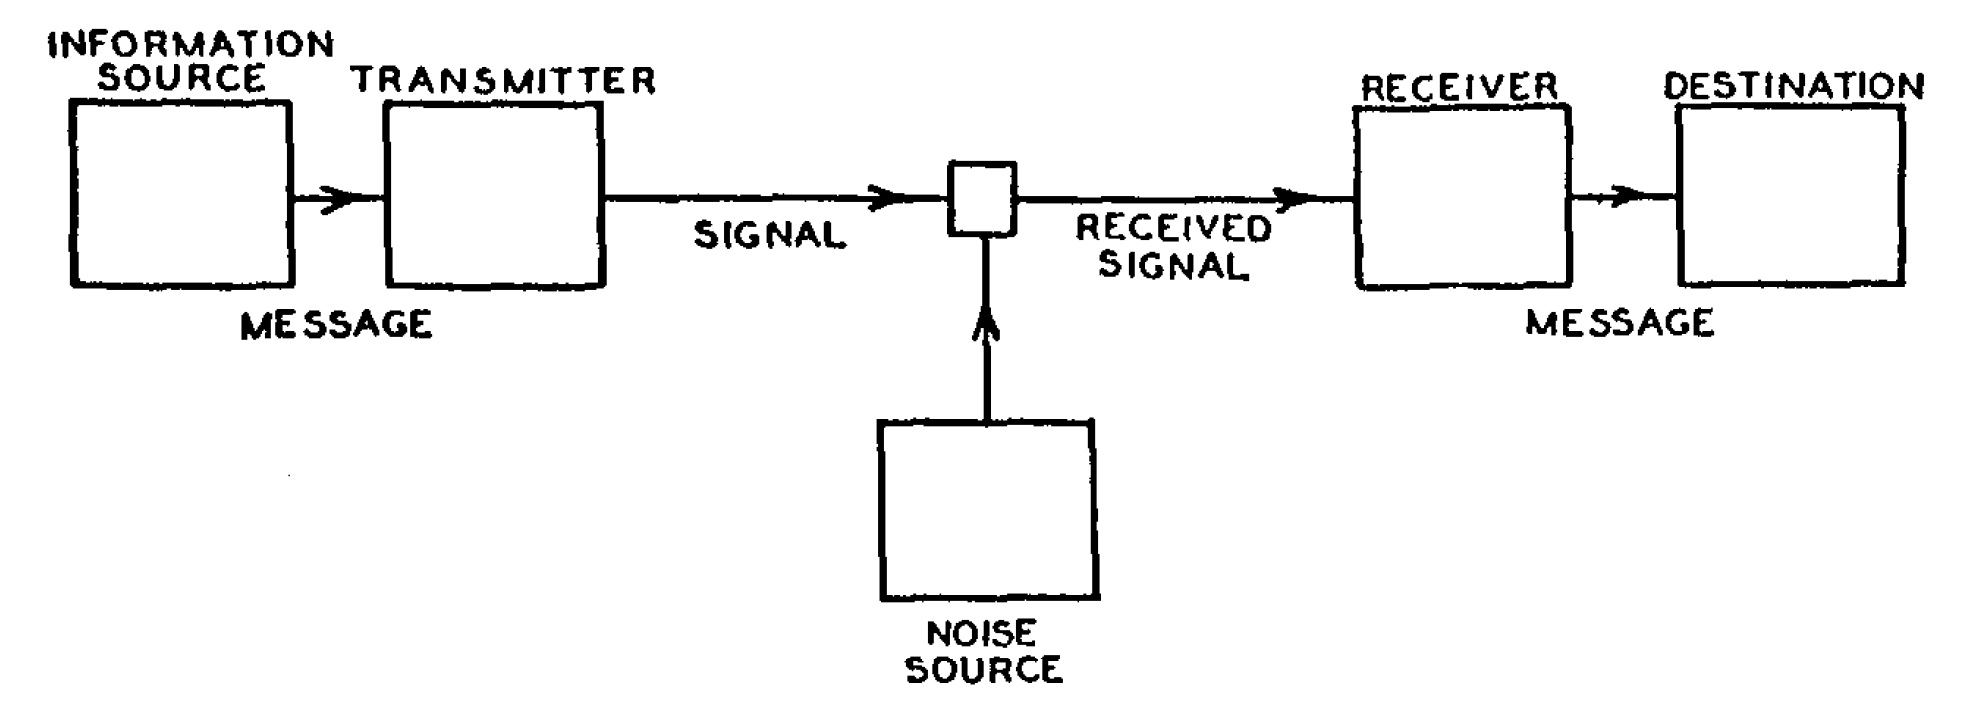
\includegraphics[width=0.8\textwidth]{figs/ch1/shannon.jpg}
\caption[A simplified block diagram of a general communication system.]{\textbf{A simplified block diagram of a general communication system.} A communication system can be abstracted as follows: an \textit{information source} produces a message to be sent through a \textit{transmitter} which converts it to a signal which can be sent via a communication \textit{channel}. The received signal is noisy and is converted back to the message by the \textit{receiver} which is then delivered to the \textit{destination}. Taken from \cite{shannon1948}.}
    \label{fig:my_label}
\end{figure}
%----------------------------------------------------
\pagebreak
%----------------------------------------------------
\begin{table}[H]
    \centering
    \caption[Table title]{\textbf{Table title.} Extended description of tables contents.}
    \begin{tabularx}{\textwidth}{>{\raggedright\arraybackslash}m{8cm}>{\raggedright\arraybackslash}X>{\raggedright\arraybackslash}X}
    \toprule[2.25pt]
    \multirow{3}{*}{\textbf{Heading 1}}        &  \multicolumn{2}{c}{\textbf{Heading 2}}   \\
    \cmidrule[0.5pt](lr){2-3}
    &  \multicolumn{1}{c}{\textit{\small Subheading 1}} & \multicolumn{1}{c}{\small \textit{Subheading 2}}\\
    &  \multicolumn{1}{c}{\small [units]} & \multicolumn{1}{c}{\small [units]}\\
    \midrule[1pt]
         &  &\\
         &  &\\
         &  &\\
    \bottomrule[2.25pt]
 \end{tabularx}

    \label{table:my_label}
\end{table}


%====================================================
\section{Problem statement}
\label{sec:ch1.problemstatement}
%====================================================
Equations are numbered and include the chapter number. As they are considered part of the text, they include punctuation, and each parameter must be described in the text below. Ensure that the units are stated and where possible use SI units. For example, the Maxwell equations are expressed as:
\begin{align}
\nabla \cdot \bm{E} &= \frac{\rho}{\epsilon_0}, \\
\nabla \cdot \bm{B} &= 0, \\
\nabla \times \bm{E} &= -\frac{\partial \bm{B}}{\partial t}, \\
\nabla \times \bm{B} &= \mu_0 \bm{J} + \mu_0 \epsilon_0 \frac{\partial \bm{E}}{\partial t},
\end{align}

where $\bm{B}$ is the magnetic flux density in T, $\bm{J}$ is the total current density in A/m$^2$, $\bm{E}$ is the electric field in V/m, $\mu_0$ is the permeability of free space (4\(\pi \times 10^{-7}\) H/m), and $\epsilon_0$ is the permittivity of free space (8.85 \(\times 10^{-12}\) C$^2$/N·m$^2$).


%====================================================
\section{Project objectives}
\label{sec:ch1.projectobjectives}
%====================================================
The \gls{gps} is used for positioning. The \gls{miz} is of particular interest in the \gls{so}.
%====================================================
\section{Scope, limitations and assumptions}
\label{sec:ch1.scope}
%====================================================
%====================================================
\section{Plan of development}
\label{sec:ch1.planofdevelopment}
\pagebreak
%====================================================
%----------------------------------------------------
%****************************************************
% END
%****************************************************

%---------------------------------------------------------------------
% Chapter 2: Literature Review
%---------------------------------------------------------------------
%=====================================================================
%   LITERATURE REVIEW
%=====================================================================
%   Replace this chapter with your own. What is here is a demonstration of
%   how to cite, kept because it is the thing people get wrong.
%
%   The keys cited below are PLACEHOLDERS from thesis.bib. They exist to show
%   the citation commands working. Do not leave them in your thesis.
%=====================================================================
\chapter{Literature review}
\label{ch:review}

%---------------------------------------------------------------------
%   HOW TO CITE
%---------------------------------------------------------------------
%   natbib gives you two forms, and they are NOT interchangeable.
%
%     \citet{key}   TEXTUAL. The author becomes part of the sentence.
%                   "As \citet{shannon1948} showed, ..."
%                   -> As Shannon (1948) showed, ...
%
%     \citep{key}   PARENTHETICAL. The whole citation sits in brackets at
%                   the end of a clause.
%                   "...is a solved problem \citep{shannon1948}."
%                   -> ...is a solved problem (Shannon, 1948).
%
%   \cite{key} behaves like \citet in author-year mode and like a numeric
%   citation in IEEE mode, so it reads differently depending on the switch at
%   the top of 0_main.tex. Prefer \citet and \citep: they always mean what
%   they say.
%
%   In IEEE mode both come out as [1], which is why IEEE citations are easier
%   to write and harder to read.
%---------------------------------------------------------------------

Textualtual, where the author is the subject of the sentence:
\citet{shannon1948} established the information-theoretic limits that still
bound modern communication systems.

Parenthetical, at the end of a clause:
The effect is well documented \citep{placeholder_article}.

Several sources at once, which natbib sorts and compresses:
The same conclusion is reached by three independent routes
\citep{placeholder_article,placeholder_book,placeholder_conference}.

A page, chapter or section within a source:
The register map is given in full \citep[Ch.~8]{placeholder_website}.

The year alone, where the sentence already names the author:
Shannon's channel capacity theorem \citeyearpar{shannon1948} is the origin of
the result.

%---------------------------------------------------------------------
%   thesis.bib ships with one example of each entry type: article, book,
%   chapter in an edited book, conference paper, thesis, technical report and
%   website. Copy the nearest one and edit it.
%---------------------------------------------------------------------


% Sea-Ice Draft is the vertical distance that sea ice extends below the waterline down to the bottom of the ice sheet or floe.

\section{Introduction}
\label{sec:ch2.introduction}
% Introduce literature review and summarise whats in it
% Roadmap for the chaptor



\section{Region importants}
\label{sec:ch2.region}
% TODO: Rename chapter
% Discussion about where MIZ is, why it matters climatically
% Why pancake / flow morphology is dominant ice type here
% Why the underside specifically matters:
% - roughness, algae, heat/momentum exhange..

% Intro sentence as to what the MIZ is, basic importance
Antarctic more defined by ice texture., important to understand the underrside of the ice

The Marginal Ice Zone (MIZ) is the portion of the ice cover between the main ice cover and open Sea, and is typically defined as the region with sea ice concentration (SiC) between 15-80\% \citep{dumontMarginalIceZone}. The MIZ is responsible for several important processes. It provides a habitat for sea-ice algea, which act as primary producers during low productivity periods \citep{lizotteContributionsSeaIce2001}, and polar sea ice acts as an carbon pump that increases the net CO\textsubscript{2} uptake through brine rejection and further processes \citep{rysgaardSeaIceContribution2011}. 

 Majority of studies regard ice thickness using to categorise the MIZ, but \citet{vichiIndicatorSeaIce2022} argues that the 15-80\% model is less effective in the southern oceans because sea ice type is unrelated to the concentration value (also explain why he says that, sat data I think). They further suggests that in the thin, seasonal frazil dominated areas, the energy exchange across the atmosphere-ice-ocean interface is more dependent on the sea ice tecture than percentage coverage. The underside of the ice is important as it defines the ICE-SEA interface and is critical important in defining drag coeffiecients (ref Hoerten et al.).

% FORMATION OF ICE?

 % Metric of coverage is less relavent in antacric, exhanges of energy more affected by sea ice texture...


\section{Current Data and Gaps}
\label{sec:ch2.existing_Data}
% What satellites gave and limitations for better understanding the underside of ice8
% What in-situ methods exist (conf papers)
% Key gap is most do under-ice thickness and acoustic reconstruction at a course scale. acoustic vs optical gap
% compare reconstruction options (sonar, structured light, laser, monocular SFm, passive stereo, stereo)
% % Interestingly ref ni https://www.cambridge.org/core/journals/annals-of-glaciology/article/development-of-sea-ice-in-the-weddell-sea/06887E8C6716177BC0491F73BF87F92C




\section{Stereo vision for Surface Reconstrucion}
\label{sec:ch2.calibration}

% EPipoplar geometry and rectificatino
% Correspondance ant matching (poor underwater)
% Pinhole camera model & Calibration
% Point clouds, registration, and fusion
% Evaluating accuracy of above
% Stereo Geometry and 3D reconstruction (in-air case, point clouds, disparity->depth)


\section{Underwater challenges and calibration techniques}
\label{sec:ch2.underwater_challenges}
% Connection back to original prohject
% Existing calibration techniques and how they compensate (S2667393226000153)
% 		- Ignore refratcion and absorb into distortion
%		- Explicit physical / ray-tracing models
%		- The Pinax modl
%		- Corrective optics
% Point to methedology chapter

% Concerns around IMU that uses magnometer in high / low lattitudes

%=======================

At its core, we need to get transfrom pixel data and measurements into metric values. This transformation is largely system dependent and calibration is required to compensate. A set of intrinsic parameters are needed to be determined \citet{semeniutaAnalysisCameraCalibration2016}:

% TODO: Make this a table and have a description / method of finding section
\begin{itemize}
	\item Pixel size
	\item Center of projection
	\item principal length
	\item distortion characteristics
\end{itemize}
 \citet{semeniutaAnalysisCameraCalibration2016}:
 

Can find these parameters by...





% INtroduce the challenges, explored solutions.




% How to now pivot to why we are using stereo cams. Is this within lit review territory?

% IF so, then air calibration, reconstrucion 
%---------------------------------------------------------------------
% Chapter 3: Theoretical development
%---------------------------------------------------------------------
%*********************************************************************
\chapter{Theoretical development}
\label{ch:theory}
%*********************************************************************

\section{Camera stuff}
\label{sec:CamCal}


% CLAUDE:
Claude thinks its important to only calibrate with gray because of somme conversion that might happen. Must have a chat and try prove this. 


% Reinhard Klgjgjgjgjgjjg
for Intrinsic (cam specific) and given extrinsic 
Ininsic: (effective) focal length, dimensions of the sensor matrix, sensor cell size or aspect ratio of sensor high to width, radial distorition paramteres, coordinates of the principal point, or the scaling factor
Extrinsic: Applied affine transorms for identifying poses (location and direction) of cameras in a world coordiantae system

Use geometric patterns on 2D or 3D accurately measered. E.g. calibration rig, 

Each new placement in the 3D scene defines a different world coordinate system

\textbf{Involved Transforms:} Mention of 5 brokendown Transforms

\textbf{Lens Distortion:} 3D-2D image points combines a perspective prohection (deivates from pinhole camera), caused by radial distortion
Gives (simplified) two equatiosn to explain 

After lens distoriton, can view each camera as a pinhole-camera model

\textbf{Designing a Calibration Method:}

Points (Xw, Yw, Zw) on the calibration rig (e.g. corders of the sequares) or calibration marks are known by their physically measured coordinats - deteremine a correspongin (x,y) if possible with sub pixel accuracy. Tat is the projection of Xy,Yw,Zw in the world plane. E.g. 100 points, 100 equations 

We can refine the camera model (e.g. different focal length in the x and y direction, f\_y, f\_x). Can also include edege length e\_x and e\_y of the sensor cells used in the sensor matrix in the camera, .... and more

The resulting equational systems become more complex but with more unkowns.

The equations defining our camera model contain  X\_Y,Y\_W,Z\_W, x and y as known calies -> intrinsic and extrinsic camera parameters as unkowns. The resulting equation system (neccessarily nonlinear due to central projection or radial distortion) needs to be solved for the specified unkowns - over determeined situations provide stability of a used numeric solution scheme

\textbf{Manufacturing a calibration board:}
Rigid B\&W pattern common, atleast 7x7 squares large enough s.t. minimum size when recorded on the image is atleast 10x10 pixels (i.e. having a camera with effective focal length \textit{f}, this allows us to estimat the size of \textit{axa} for each square assuming a distance of b m between camera and board. 

\textbf{Localising Corners in the Checkerboard}
 Calibration marks are the corners of squares (aprox by the intersection points of grid lines, thus defining corners potentially with sub pixel acccuracy). 
 
 Mention of the HOugh space method for detecting line segments, requires that lens distortion has been removed from recorded images prior to applying the Hough-Space method. IMages with lens distortion will show bended lines rather than straight grid lines. 
 
 \textbf{Localising Calibration marks}
 Can also be defined by circular or square dots. Popular if same location, can be permanently painted on walls or other static surfaces.
 
 Supbixel accuracy by calculating the centroid of this region (example given)
 
 \textbf{Rectification of Stereo Image Pairs:}
 Main complexity is to identify correspoinding points in pairs of input images recorded by two cameras. (See chapter 8). Convenient to warp the image pairs so it appears they are recorded in canonical stereo (by a pair of identical cmeras) -> called geometric rectification)
 
 \textbf{IMPORTANT STUFFA BOUT THE CAMERA MATRIX}
 - More interesting stuff on structured lighting 
 
 
 \textbf{STEREO MATCHING CHAPTER 8}
 \textbf{Matching, Data Cost, and Confidence}
 Stereo matching is an example of labelling approach of sec 5.3.1. 
 Labelling function\textit{f} gives label f\_p E L (a disparity) to each pixel location pE$\Omega$m applying error functions E\_{data} and E\_{smooth}... ref sec 5.30
 
  Accumulated costs of label .. are the combined data and adjacent smoothness error valies 
  
  Different types of cost function options, specified as \textit{E\_{data}}
  
  Interesting image showing Stereo pair crossing
  
  Kind of like neighbourhood of pixels as box, compared on an epipolar line (same row due to canoical stero geometry).
  
  \textbf{Generic Model for Matching}
  L and R image, one is now base and othe ris match image (B,M). For pixel (x,y,B(x,y)) in base image, searh  for corresponding (x+d,y,M(M(x+d,y)) in match image). - ON same epipolar line. 
  
  \textbf{Base and Match Images and Search Intervals:}
  d ends up being the diff betweeen on epipolar basically
  
  \textbf{Label Set for Stereo Matching}:
  Assumes right-to-left matching to avoid +/- switching. End up with label set L={-1,0,-1,...-d\_{max}}. Using intrin and extrin of camera param, d\_{max} can be estimated by the closest objects in the scene that are "still of interest". 
  
  \textbf{Neighbourhoods of correspondants}
 Issues with SSD (Squared sum of differences) or SAD( Absolute differenceS), justifies 3D Cost Matrix
 \textbf{3D Data Cost Matrix}
 Some fun maths
 Compresenive repr of all the involved data costs -> can be used for further optimisation (using smoothness-cost function in the control of the \textit{stereo} matching)

 
 \textbf{Data cost functions
 	Gives list of cost functions:
 	\begin{itemize}
 		\item Zero-Mean version
 		\item NCC Data Cost
 		\item The Census Data-Cost Function
 	\end{itemize}
 	
 	
 \textbf{From Global to Local Matching}
 INtroduces SGM which is key for openCV, easy linkage
 
 Justification for OPENVC Over MATLAB w.r.t more SGM knobs.
 	
 	
 	
 	
%================================
\section{Camera Calibration}

 
% https://storage.googleapis.com/docs-product-files/stellarHD-series/stellarHD/datasheets/stellarHD-datasheet.pdf


% One of these;
% https://www.ovt.com/products/#image-sensor?is_technology=omnipixel3-gs


% What lenses we have + Stats
% How they are optically calibrated, results in different FOV in air and in water...
% 
% 
 	
The StellarHD cameras are paired with Aquagon lenses. These lenses compensate for .. using a 7 lense elements (2 aspherical and 2 extra-low dispersion). 
\textbf{Aquagon Lens details:}
 \begin{itemize}
 	\item Fixed Focus
 	\item 3.0mm Focal Length
 	\item f/1.6 Aperture
 	\item 25cm Minimum Focus distance
 	\item Distortion <-1.5\% (Measured how?)
 	\item Back Focal Length 2.05mm
 	\item IR Filter 650nm
 	\item Horizontal FOV (78 degrees)
 	\item Vertical FOV 67)
 	\item Diadonal FOV 93
 \end{itemize} 	
 
 \textbf{Sensor Specifications}
 \begin{itemize}
 	\item 1/2.9” Omnivision OmniPixel 3-GS™ CMOS Sensor
 	\item Pixel Size 3 µm (H) × 3 µm (V) 
 	\item Global Shutter
 	\item Max Resolution 1600x1200
 	\item YUY2, MJPEG Compression formats
 \end{itemize}
 	
 % COmpariso
 
 HYPERFOCUS for fixed focus lens, foxed from then onwards
 	
The Aquagon quotes it's FOV values as in water readings. While these FOV values are extracted during camera calibration, the choice of calibration method is somewhat dependent on the cameras setup (i.e is it Wide-angle). 

Go down non-wide angle calibration mode

Compare different algorithms and which applications to do it in.

% Comparison of software: https://www.mdpi.com/1424-8220/24/20/6595

Although the Aquagon lenses have been specifically designed to adjust for underwater effects, in air calibration is still an important part of the testing process as a point of reference and to better understand the calibration process in a controlled environment. This calibration testing took place within ARU's Experimental laboratory under artificial lighting conditions.

Common calibration techniques implement checkrboards as explained in SECTION X. Due to the difficulties (leaning off boat) in underwater in-situ calibration, it was chosen to use calibration boards with fiducial markers. Fudicial markers are "landmarks" to aid in computer vision models. Unique IDs are "encoded in their structure following a pre-defined pattern system and provide a means to implement reliable pose estimation of the marker with respect to the camera.". 


% FOR LIT REVIEW:
"degradation factors, such as lighting intensity attenuation, back scattering, forward scattering and macroscopic floating particles"

"Due to these effects, underwater images generally present low contrast, non-uniform lighting, blurring and noise [19]."

\cite{dossantoscesarEvaluationArtificialFiducial2015} compared different fiducial markers in an underwater tanks across  six turbitiy ? and 2 lighting conditions. They compared ARToolKit, AprilTags, ArUco and found that AprilTags were able to detect smaller targers across all turbifiry, lighting levels aswell as at larger angles. Found to be comnputationally the slowest, not an issue here. Ideally test myself but dont have tiem.

Chose to go with AprilGrid

"Bio-optical sensors measuring light scattering and particulate backscatter record these temporary biological blooms as modest turbidity spikes in the range of ~1 to 3 NTU (Garcia et al., 2020; Schallenberg et al., 2019)"


DEsign around Turbidity of 3 NTU

Deciding size of board: 
Using their data collected for 3.6 FTU. 

Minimum focus distance of 25cm

How to determine which board size (cxc) to go withg tho. 

Choosing apriltag for worst case scenario.

Paper expresses detected marker size in pixels. At FTU of 3.6, detected marker size as low as 21 pixels. 

After too much ua[[ing, claude gace me one:]
family:      tag36h11
tag size:    0.150 m   (black square, outer edge)
plate size:  0.190 m   (adds 1-cell white quiet zone each side)
IDs:         0-3 (or however many targets you need)
max_hamming: 0
resolution:  1600x1200
range:       0.3 - 2.0 m



Looking 

% CLaude and paper to determnie minimum noard size.

% DETERMINING CHARU BOARD SIZE AND MATERIAL
Dibont - give reference for why, comment on shrinkage
Type of DIbon offered by orms - give reference for which
Size - give reference for why

CLAUDES COMMENTS ON THE BOARD CHOICE:
Dont do brushed aluminum - aluminum shows through all whire areas of the image - white squares bare metal, low contrast under lights. Bad for corner detectrion at an angle. Rather smooth white powder coated

Claude thinks A2 (420x695) is the sweet spot. More managable

Need a custom quore - dont want the wood sub frame , will swell and delaminate. Ask for bare panel or drill mounting holes

Seal the cut edgfes - Dibond is two aluminum skins over a polyethylene core. Seawater might cause rust in the aluminum / PE vrevace. A bead of epoxy will do the tick.

Ask about the gloss levels of the UV inks. Tent towards semi glossy, if we can do it matte, lets fo it.

Ask about printer accuracy

Use white not aluminum, aluminium reflective different at different angles




I'll use tag36h11 because standrdand what they used in the report comparison. 
We want to have 30-50mm white boarder to avoid merging of background into tag boardrs

Underwater required picels above 25-pixel rule the minimum pixel size required for reliable detection increases significantly. Therefore, the 25-pixel rule used in air is a absolute lower bound; underwater, you should aim for 40 to 60+ pixels per tag to maintain subpixel corner accuracy.


We want to work with 1-2 meters calirated.

Pin-Hole Model Pixel CalculationThe pixel width $p$ of a tag in the image plane depends on tag size $S$ (meters), distance $D$ (meters), and focal length $f_x$ (pixels):$$p = \frac{S \cdot f_x}{D}$$For a standard camera underwater (assuming a $60^\circ$ to $70^\circ$ horizontal field of view in water due to flat-port refraction), focal length $f_x$ typically ranges between 1200 and 1400 pixels for a 1600-pixel wide sensor. Assuming an average focal length $f_x = 1300\text{ pixels}$:Option A: $65\text{ mm}$ Tag Size ($S = 0.065\text{ m}$)At 1 meter: $p = \frac{0.065 \cdot 1300}{1.0} \approx \mathbf{84.5\text{ pixels}}$ (Excellent detection)At 3 meters: $p = \frac{0.065 \cdot 1300}{3.0} \approx \mathbf{28.1\text{ pixels}}$ (Slightly low for underwater contrast)Option B: $85\text{ mm}$ Tag Size ($S = 0.085\text{ m}$)At 1 meter: $p = \frac{0.085 \cdot 1300}{1.0} \approx \mathbf{110.5\text{ pixels}}$ (Excellent detection)At 3 meters: $p = \frac{0.085 \cdot 1300}{3.0} \approx \mathbf{36.8\text{ pixels}}$ (Safe margin for underwater blur)




% ===== ATTEMPT 2 FOR BOARD SIZE

April tag size:
 QR tag comprise about
268 pixels (not including required headers or the payload),
whereas the visual fiducials described in this paper range
from about 49 to 100 pixels, including the payload.
% https://april.eecs.umich.edu/pdfs/olson2011tags.pdf



Underwater turbidity:
In order to evaluate the capability of the marker systems to detect small markers in turbid underwater environments, the camera is centered in front of the markers and then moved further away, increasing the distance between the camera and the markers and therefore decreasing the marker size in pixels

We're going with minimum of 40 pixels fo rmax turbidity situation


I ended up choosing one based on the online sold one and also 50mm size of tag from underwater testing


 

 
 
 %============================================ 3D Reconstruction comparison ============
 
%*********************************************************************
 
 
 
 
 
 
%---------------------------------------------------------------------
% Chapter 4: Design description
%---------------------------------------------------------------------
%*********************************************************************
%	PROPOSED DESIGN
%*********************************************************************
\chapter{Design description}
\label{ch:design}
%---------------------------------------------------------------------

%*********************************************************************
% End of Design
%*********************************************************************
%---------------------------------------------------------------------
% Chapter 5: Experimental design
%---------------------------------------------------------------------
%*********************************************************************
%	CHAPTER 5 - EXPERIMENTAL PROCEDURE
%*********************************************************************
\chapter{Experimental procedure}
\label{ch:experiments}
%---------------------------------------------------------------------

%=====================================================================
\section{Experimental setup}
\label{sec:ch5.setup}
%=====================================================================
% Rig, tank, lighting, turbidity control, ground truth measurement


%=====================================================================
\section{Experiment 1: Stereo calibration in air and underwater}
\label{sec:ch5.exp1_calibration}
%=====================================================================
% Calibration tests (in air vs underwater)
Initial underwater tests were done into the sun, not at full quality (oops).
This resulted in minimal detection and an initial default detection of ...


%=====================================================================
\section{Experiment 2: Reconstruction of known objects}
\label{sec:ch5.exp2_knownobjects}
%=====================================================================


%=====================================================================
\section{Experiment 3: Upward-facing reconstruction of a sea ice model}
\label{sec:ch5.exp3_seaice}
%=====================================================================

%*********************************************************************
% END
%*********************************************************************

%---------------------------------------------------------------------
% Chapter 6: Results
%---------------------------------------------------------------------
%*********************************************************************
%	RESULTS
%*********************************************************************
\chapter{Results}
\label{ch:results}
%---------------------------------------------------------------------

%*********************************************************************
%---------------------------------------------------------------------
% Chapter 7: Discussion
%---------------------------------------------------------------------
%*********************************************************************
%	CHAPTER 7 - DISCUSSION
%*********************************************************************
\chapter{Discussion and analysis of pipeline performance}
\label{ch:discussion}
%---------------------------------------------------------------------

%*********************************************************************
% END
%*********************************************************************

%---------------------------------------------------------------------
% Chapter 8: Conclusions
%---------------------------------------------------------------------
%*********************************************************************
%	CHAPTER 8 - CONCLUSIONS AND RECOMMENDATIONS
%*********************************************************************
\chapter{Conclusions and recommendations}
\label{ch:conclusions}
%---------------------------------------------------------------------

%=====================================================================
\section{Conclusions}
\label{sec:ch8.conclusions}
%=====================================================================


%=====================================================================
\section{Recommendations for further work}
\label{sec:ch8.furtherwork}
%=====================================================================

%*********************************************************************
% END
%*********************************************************************

%---------------------------------------------------------------------
% Chapter 9: Recommendations
%---------------------------------------------------------------------
\include{9_furtherwork}
%   Marks the last page of the body. Everything after this (appendices,
%   bibliography) is excluded from the page count.
\label{body:end}
%---------------------------------------------------------------------
% Appendices
%---------------------------------------------------------------------
\appendix
%---------------------------------------------------------------------

\renewcommand{\thechapter}{\Alph{chapter}} % Makes chapters A, B, C, etc.
\renewcommand{\thesection}{\thechapter.\arabic{section}} % Makes sections A.1, A.2, etc.
\renewcommand{\thesubsection}{\thesection.\arabic{subsection}} % Makes subsections A.1.1, A.1.2, etc.

% Reset section counter at the beginning of each appendix chapter
\setcounter{section}{0}
%---------------------------------------------------------------------


%---------------------------------------------------------------------
% Appendix A
%---------------------------------------------------------------------

\chapter{GitHub repository}
%\addcontentsline{toc}{chapter}{Appendix A: GitHub repository}

This appendix provides a link to the GitHub repository where the code and additional materials for this \documenttype\ can be found.

\section{Title for appendix A.1}

\begin{itemize}
    \item GitHub Repository: \gitrepo
\end{itemize}

%---------------------------------------------------------------------
%ADD THE READ ME HERE

%---------------------------------------------------------------------

%---------------------------------------------------------------------
% Appendix B
%---------------------------------------------------------------------

\chapter*{Appendix B: Ethics approval}
\addcontentsline{toc}{chapter}{Appendix B: Ethics approval}


%\includepdf[pages=-]{path/to/your/file.pdf}


%---------------------------------------------------------------------
%

%---------------------------------------------------------------------
%---------------------------------------------------------------------
%   C: the original topic description, as issued during project selection.
%      Required for a final year project report. Not usually included in a
%      postgraduate thesis: comment it out if you are writing one.
%
%   D: the ECSA Graduate Attributes reflection table. Required for a final
%      year project report, since ECSA accreditation depends on it. Not
%      required for a postgraduate thesis.
%---------------------------------------------------------------------
%=====================================================================
%   APPENDIX C: TOPIC DESCRIPTION
%=====================================================================
%   The topic description as it was issued during project selection, before
%   the problem was refined.
%
%   Required for a final year project report. Not usually included in a
%   postgraduate thesis: comment out %=====================================================================
%   APPENDIX C: TOPIC DESCRIPTION
%=====================================================================
%   The topic description as it was issued during project selection, before
%   the problem was refined.
%
%   Required for a final year project report. Not usually included in a
%   postgraduate thesis: comment out %=====================================================================
%   APPENDIX C: TOPIC DESCRIPTION
%=====================================================================
%   The topic description as it was issued during project selection, before
%   the problem was refined.
%
%   Required for a final year project report. Not usually included in a
%   postgraduate thesis: comment out \include{C_topicdescription} in
%   0_main.tex if you are writing one.
%
%   HOW TO USE THIS
%     1. Put the PDF of the topic list in pdfs/.
%     2. Uncomment the \includepdf below and set the page range to YOUR topic.
%
%   Nothing is included by default, because the PDF is specific to a course
%   and a year and does not belong in a template. Leaving a hardcoded
%   \includepdf here would break the build for everyone who cloned the repo
%   without that file.
%=====================================================================

\chapter*{Appendix C: Topic description}
\addcontentsline{toc}{chapter}{Appendix C: Topic description}
%---------------------------------------------------------------------
The original topic description used during the project selection process is
included below. This topic has since been further refined, and the exact
problem that was investigated is described in
Section~\ref{sec:ch1.problemstatement}.

%---------------------------------------------------------------------
%   Include YOUR topic description here. One \includepdf, with the page
%   range of your topic in the topic list.
%
%   \includepdf[pages=2-5]{pdfs/topics.pdf}
%---------------------------------------------------------------------
 in
%   0_main.tex if you are writing one.
%
%   HOW TO USE THIS
%     1. Put the PDF of the topic list in pdfs/.
%     2. Uncomment the \includepdf below and set the page range to YOUR topic.
%
%   Nothing is included by default, because the PDF is specific to a course
%   and a year and does not belong in a template. Leaving a hardcoded
%   \includepdf here would break the build for everyone who cloned the repo
%   without that file.
%=====================================================================

\chapter*{Appendix C: Topic description}
\addcontentsline{toc}{chapter}{Appendix C: Topic description}
%---------------------------------------------------------------------
The original topic description used during the project selection process is
included below. This topic has since been further refined, and the exact
problem that was investigated is described in
Section~\ref{sec:ch1.problemstatement}.

%---------------------------------------------------------------------
%   Include YOUR topic description here. One \includepdf, with the page
%   range of your topic in the topic list.
%
%   \includepdf[pages=2-5]{pdfs/topics.pdf}
%---------------------------------------------------------------------
 in
%   0_main.tex if you are writing one.
%
%   HOW TO USE THIS
%     1. Put the PDF of the topic list in pdfs/.
%     2. Uncomment the \includepdf below and set the page range to YOUR topic.
%
%   Nothing is included by default, because the PDF is specific to a course
%   and a year and does not belong in a template. Leaving a hardcoded
%   \includepdf here would break the build for everyone who cloned the repo
%   without that file.
%=====================================================================

\chapter*{Appendix C: Topic description}
\addcontentsline{toc}{chapter}{Appendix C: Topic description}
%---------------------------------------------------------------------
The original topic description used during the project selection process is
included below. This topic has since been further refined, and the exact
problem that was investigated is described in
Section~\ref{sec:ch1.problemstatement}.

%---------------------------------------------------------------------
%   Include YOUR topic description here. One \includepdf, with the page
%   range of your topic in the topic list.
%
%   \includepdf[pages=2-5]{pdfs/topics.pdf}
%---------------------------------------------------------------------


%---------------------------------------------------------------------
% Appendix D
%---------------------------------------------------------------------

\chapter*{Appendix D: ECSA Graduate Attributes}
\addcontentsline{toc}{chapter}{Appendix D: ECSA Graduate Attributes}
%---------------------------------------------------------------------

\section*{Project mapping to ECSA Graduate Attributes}
\addcontentsline{toc}{section}{Project mapping to ECSA Graduate Attributes}

The table below provides a structured reflection on where each of the required \gls{ga} as defined by \gls{ecsa} associated with the final year project is met. This includes reference to the specific Chapter/Section (where applicable). 

\vspace{1em}


{\small
\renewcommand{\arraystretch}{1.5}
\begin{longtable}{>{\raggedright\arraybackslash}p{0.05\textwidth} >{\raggedright\arraybackslash}p{0.25\textwidth} >{\noindent\justifying\arraybackslash}p{0.6\textwidth}}
\toprule
\textbf{GA} & \textbf{Graduate Attribute Description} & \textbf{Student reflection: How this outcome was achieved during the project} \\
\midrule
\endhead

GA1 & \textit{Problem solving} & \\
\cmidrule(lr){1-3}
GA4 & \textit{Investigations, experiments and data analysis} & \\
\cmidrule(lr){1-3}
GA5 & \textit{Use of engineering tools} & \\
\cmidrule(lr){1-3}
GA6 & \textit{Professional and technical communication} & \\
\cmidrule(lr){1-3}
GA8 & \textit{Individual and collaborative teamwork} & \\
\cmidrule(lr){1-3}
GA9 & \textit{Independent learning ability} & \\
\bottomrule
\end{longtable}
}






%=====================================================================
%	BACK MATTER
%=====================================================================
\backmatter
%---------------------------------------------------------------------
% Bibliography
%---------------------------------------------------------------------
%---------------------------------------------------------------------
%   BIBLIOGRAPHY STYLE
%---------------------------------------------------------------------
%   Driven by \ifIEEEcite, set once at the top of this file.
%
%   plainnat  natbib's author-year style. Part of natbib itself, so always
%             available, and it matches the Harvard convention the
%             declaration page commits you to.
%
%   IEEEtran  the IEEE numeric style. Ships with the IEEEtran package.
%
%   NOTE: this was previously \bibliographystyle{kluwer}. kluwer.bst is not
%   part of TeX Live and was not in this repository, so bibtex failed with
%
%       I couldn't open style file kluwer.bst
%
%   and no bibliography was produced at all. If your department supplies a
%   kluwer.bst, commit it alongside 0_main.tex and use it here.
%---------------------------------------------------------------------
\ifIEEEcite
    \bibliographystyle{IEEEtran}
\else
    \bibliographystyle{plainnat}
\fi
{\small \bibliography{thesis,zotero_collection}}
\addcontentsline{toc}{chapter}{Bibliography}
%---------------------------------------------------------------------
\end{document}
%---------------------------------------------------------------------
%	End of the document
%=====================================================================


